\chapter{Methods}
\label{chapter3}
Within this chapter, we describe our method. We begin by discussing the motivations for our method, which are grounded in human reasoning, then we formalise our method and supply an illustrative example. We finish by discussing the various implementations that were produced in order to evaluate the main contribution of our method.

\section{A Human Thought Process}
When human's make decisions, they are often driven by previous experiences and some form of internal model of the world that we maintain. However, sometimes we question ourselves and think "what if this other decision is better?"; this leads to us making different decisions, which are driven by reasoning. As an example, consider the route that you travel to work everyday. At some point you might question yourself and think "what if there is a faster route?", which may lead to you taking a longer route, by distance, because you think that there is a possibility that it could be faster. It might turn out that the longer route is indeed slower, and you may never try it again. However, it might be that you realise that the longer route is much faster, due to lack of congestion for example, and thereafter you follow it every morning. This is the decision-making and reasoning process that we try to emulate.
\section{Unifying Optimism and Intrinsic Motivation}
We propose a framework that synthesises planning and reinforcement learning that aims to achieve efficient exploration through optimism and intrinsic motivation. We acknowledge that model inaccuracies are inevitable, but inaccurate models are still useful, and use this as a basis to drive exploration. We enable the planner to hypothesise changes to the model that would be most beneficial to it. The planner produces plans with these hypotheses in mind, and the correctness of them is realised through experience in the real environment, leading to the model being updated accordingly.
\\This approach utilises the principle of \textit{optimism in the face of uncertainty}; we state that until we have gained experience in the environment, we are uncertain about our model, and thus we make optimistic hypotheses about the environment. Furthermore, this approach is based on intrinsic motivation; the planner has some intrinsic motivation to seek out states it is uncertain about. However, extrinsic rewards are also considered, as the planner always produces plans with maximising the cumulative reward in mind.
\\We enable the planner to make these hypotheses by equipping it with additional actions, which we denote Meta Actions. The use of Meta Actions is the main contribution of this work.

\section{Meta Actions}
\label{sec:31}
These actions do not cause the agent to act in and affect the environment, and thus do not return any observation in terms of a new state and a reward, but rather cause changes directly to the model when called upon. An important factor and one of the main difficulties is deciding what Meta Actions should be exposed to the planner and when the planner should be able to invoke the Meta Actions. Therefore, we state three conditions which all must hold for a Meta Action to be invoked: a Meta Action must be admissible, feasible and reasonable.

\begin{defn}
\label{defn:admissible}
    A Meta Action is admissible if applying it to the model leads to a better policy with respect to the model.
\end{defn}
It's important that hypothesised changes are optimistic; that they benefit the planner in some way, otherwise they are not very useful. Thus, admissibility is important, as defined in Definition \ref{defn:admissible}, if applying a Meta Action does not result in any benefit to the planner, but rather it negatively affects the planner, then it should not be called. This means that planning must be done with finding the sequence of actions that maximises reward in mind.
\begin{defn}
\label{defn:feasible_deterministic}
In a deterministic domain, a Meta Action is feasible if the target state-action pair that it is to be applied to has not been previously observed nor has that Meta Action been previously called on it.
\end{defn}
\begin{defn}
\label{defn:feasible_stochastic}
In a stochastic domain, a Meta Action is feasible if either:
\begin{itemize}
    \item The target state-action pair that it is to be applied to has not been previously observed within the current episode nor has that Meta Action been called on it within the current episode.
    \item The target state-action pair that it is to be applied to has not been previously observed within the current or previous $N$ episodes, nor has that Meta Action been called on it within the current or previous $N$ episodes.
\end{itemize}
\end{defn}
If the agent were to make hypothesises that contradict its own observations, it would induce hallucinatory behaviour. Furthermore, by the optimistic nature of our approach, its possible that the agent could infinitely hypothesise changes to the model, namely in the form of increased rewards. Therefore, feasibility is important, as defined in Definitions \ref{defn:feasible_deterministic} and \ref{defn:feasible_stochastic}. Within deterministic settings the transitions and rewards that the agent observes are the true ones; thus we can be certain that the model is correct with respect to the observations of the agent, hence Definition \ref{defn:feasible_deterministic} ensures that observations in the entire lifetime of the agent are not contradicted. Definition \ref{defn:feasible_stochastic} gives two alternate conditions for feasibility in stochastic settings, each of which are explored throughout the implementations to see which is stronger. This definition ensures that the agent cannot contradict recent observations (those within the current or previous $N$ inclusive episodes), and thus hallucinate, whilst ensuring that changes to the model cannot be infinitely hypothesised. It allows Meta Actions to be called multiple times on state action pairs, including those of which have been previously observed, this is because we can never be completely certain of the correctness of the model due to the aleatoric uncertainity introduced due to the stochasticity.

% Definition \ref{defn:feasible_deterministic} ensures that in deterministic settings the agent cannot contradict its observations, and thus hallucinate, whilst ensuring that changes to the model cannot be infinitely hypothesised.

\\
\begin{defn}
\label{defn:reasonable}
A Meta Action is reasonable if it has been embedded by-hand or learned through experience.
\end{defn}
Often, the change to the model that would be of most benefit the planner, is to simply add a transition from the current state to the goal state. However, this is almost never going to be a change that is realised to be correct, it is too optimistic, and instead would lead to behaviour akin to taking a random-walk through the state space until the goal is reached and the Meta Actions have been exhausted, or perhaps it would induce exploration that is akin to R-MAX or OIM. Hence, reasonability, as defined in Definition \ref{defn:reasonable} is key.
\section{Framework}
We assume that the environment has a discrete state space, $S$, or a state space that can be discretised, a finite action space, $A$, with deterministic or stochastic dynamics which can be described by a transition function, $T$, and deterministic rewards which can be described by a reward function, $R$. Therefore, we assume that the environment can be modelled as an MDP $E = (S, A, T, R)$, within which the agent acts at discrete time steps. The goal of the framework is to produce a policy, $\pi^*$ which maximises the cumulative reward received when acting in the environment $E$.
Additionally, we assume that an attempt at modelling the environment has been made and embedded in an MDP $M = (S, A, T', R')$, where the same conditions hold for $T'$ and $R'$ as for $T$ and $R$. We do not expect or require $M$ to be accurate. 
\\We perform model-learning by maintaining $T'$ as a \textit{tabular maximum likelihood model}, and keep track of observed transitions using a function $n$ which maps state-action-state triples to an integer indicating how many times that transition has been observed. We chose this approach of model-learning, as we assumed a discrete/discretised state space and this method offers a simple implementation of model-learning.
\\We learn a tabular Q-Function, $Q$, through Q-Learning, which the policy $\pi$ is derived from. Q-Learning was chosen over SARSA, since it allows the optimal policy to be learnt independently of the current policy being followed; this suited our framework well, since we acknowledge that the policies followed during the exploration may not be optimal.
% The choice of initialisation open.
\\Our framework consists of two distinct phases: a planning phase where exploration takes place and a model-free phase. Since we only consider episodic tasks, the agent is given a finite number of episodes, $N_p$, for the planning phase, thereafter until termination 
% (some finite number of episodes has been completed)
, the model-free learning takes over and the idea is that given sufficient model-free episodes $Q$ can converge to $Q^*$, and thus $\pi^*$ can be derived. Algorithm \ref{alg:framework_pc} gives a relatively high-level overview of the framework.


\begin{algorithm}
\caption{High-level Framework Pseudocode}
\label{alg:framework_pc}
\begin{algorithmic}
\REQUIRE $N$, number of episodes
\REQUIRE $N_p$, number of planning episodes
\REQUIRE $M=(S,A,T,R)$, model
\REQUIRE $s_s$, $s_g$, start, goal state
\ENSURE $\pi$, final policy
\STATE $Q(s,a) \leftarrow 0 $, $\forall s \in S$, $\forall a \in A$
\STATE $s \leftarrow s_s$
\FOR{$i=0$ to $N$}
    \STATE $Planning \leftarrow (i < N_p)$
    \WHILE{$s \neq s_g$}
        \IF{$Planning$ is \TRUE}
            \STATE $a \leftarrow$ Plan($s$, $s_g$)
        \ELSE
            \STATE $a \leftarrow \argmax_a Q(s,a)$
        \ENDIF
        \STATE Take action $a$ in state $s$, observe reward $r$ and new state $s'$
        \STATE Learn $Q$ according to observation.
        \IF{$Planning$ is \TRUE}
            \STATE Learn $M$ according to observation.
        \ENDIF
        \STATE $s \leftarrow s'$
    \ENDWHILE
\ENDFOR
\STATE $\pi(s) \leftarrow \argmax_a Q(s,a), \forall s \in S, \forall a \in A$
\RETURN $\pi$
\end{algorithmic}
\end{algorithm}

\subsection{The Planning Phase}
The planning phase has three distinct steps: planning, acting and learning, which can be seen in Figure \ref{fig:planning_phase}. The goal of the planning phase is to perform exploration, and provide a good estimate for $Q^*$ which the model-free learning can bootstrap and derive a policy from.

\subsubsection{Planning}
The planner constructs a temporary model, $M'$, which is identical to $M$. It then plans on $M'$ to produce a plan, $P$, from the current state $s$ to some goal, terminal, state $s_g$. The planner has access to the action space, $A$, as well as the additional Meta Actions. Whilst considering the Meta Actions, the planner may create additional temporary models, in order to evaluate the benefit of calling a particular Meta Action. If a Meta Action is chosen, then the temporary model $M'$ is updated, and planning continues. $P$ is maintained by the planner until $M$ is updated, when re-planning occurs. This ensures that unnecessary planning does not take place, saving on computational costs. However, this means that some mechanism needs to be in place for determining if the model has been altered since the last plan was generated; this can be a simple Boolean flag. $P$ is stored in a first-in, first-out (FIFO) data structure, such as a Queue. Thus, when the planner is invoked by the agent it simply removes and returns the top action.
\subsubsection{Acting}
At discrete time steps, $t$, the agent samples an action $a$ from the Planner, and executes it. If the action is a Meta Action, then it does not result in any interactions with the environment, and thus no observations or "time steps" are made. Otherwise, at time $t+1$ it observes its new state $s'$ and the scalar reward signal.
\subsubsection{Learning}
Learning only occurs of the action taken was not a Meta Action. The observation table is updated with the observed transition: $n(s, a, s') \leftarrow n(s, a, s')+1$, and if necessary the transition function, $T'$ of $M$ is updated by Equation \ref{eqn:tmlmupdate}. Furthermore, the reward function, $R'$, of $M$ is updated with the received reward, if necessary. $Q$ is updated according to the new state and reward received using Equation \ref{eqn:qlearningupdate}.

\subsection{The Model-Free Phase}
The model-free phase has two distinct steps: acting and learning, which can be seen in Figure \ref{fig:model_free_phase}. The goal of the model-free phase is to use pure model-free learning to bootstrap from the Q values learned during exploration, and get as close as possible to $Q^*$, so that $\pi^*$ can be derived.

\subsubsection{Acting}
At discrete time steps, $t$, the agent greedily selections an action $a$ with respect to the $Q$, it selects the action according to the current policy, and executes it. At time $t+1$ it observes its new state $s'$ and the scalar reward signal.
\subsubsection{Learning}
$Q$ is updated according to the new state and reward received using Equation \ref{eqn:qlearningupdate}. Eventually, the updates will not result in changes to the policy, $\pi$, and therefore it will be continually followed until termination.

\begin{figure}[h!]
    \centering
    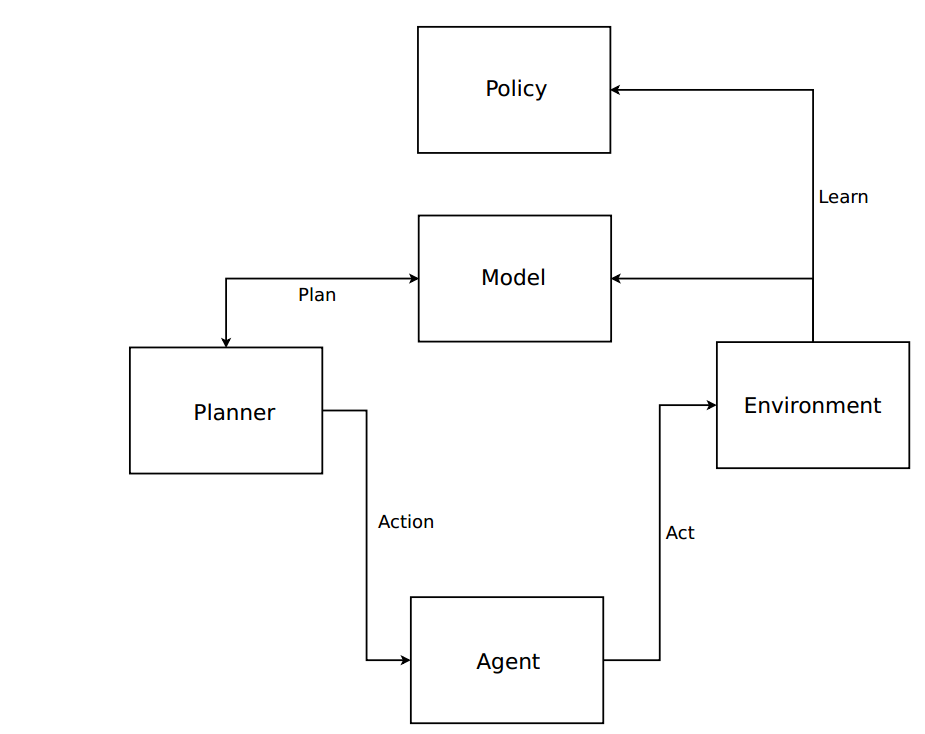
\includegraphics[max size={350pt}{350pt}]{report/assets/planning_phase.png}
    \caption{Planning Phase}
    \label{fig:planning_phase}
\end{figure}
\begin{figure}[h!]
    \centering
    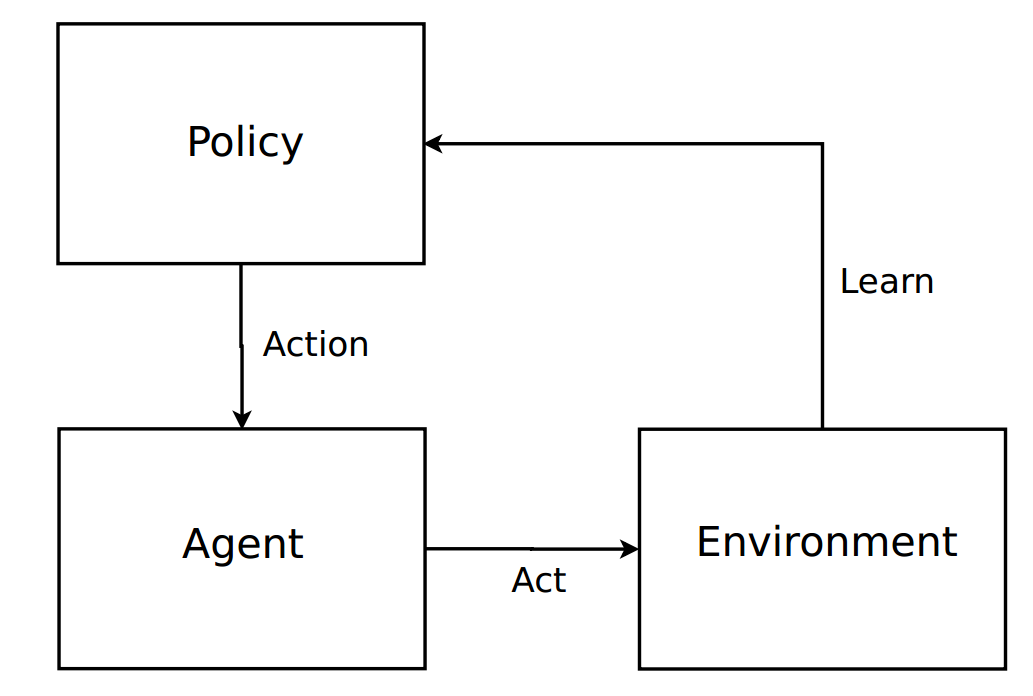
\includegraphics[max size={250pt}{250pt}]{report/assets/model_free_phase.png}
    \caption{Model-Free Phase}
    \label{fig:model_free_phase}
\end{figure}


\section{An Illustrative Example}
Consider the deterministic domain in Figure \ref{fig:cliff-real}. This is a modified version of the cliff-walking domain \cite{Sutton1998}. The red circle located at (0,0) is the agent; the goal is located in the bottom right corner, (0, 7). If the agent transitions into one of the "cliff" states, they are returned to the start state. Let's suppose that for some reason, perhaps due to changes in the environment, the agent is seeded with the inaccurate model shown in Figure \ref{fig:cliff-model}. A pure planning approach would fail, as it would continually plan a path that goes through the cliff, due to the inaccurate model. A pure model-free learning approach would probably be successful, as this is a very simple domain, however in reality domains can be much more complicated than this; which is where model-free methods begin to struggle.


% \begin{figure}
% \centering
% \begin{subfigure}{.5\textwidth}
%     \centering
%     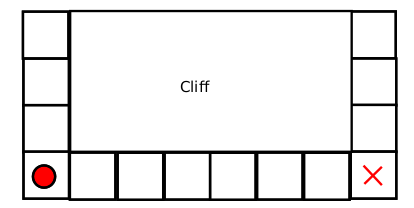
\includegraphics[max size={200}{200}]{report/assets/envs/cliff_real.png}
%     \caption{Modified Cliff-Walking Domain}
%     \label{fig:cliff-real}
% \end{subfigure}%
% \begin{subfigure}{.5\textwidth}
%   \centering
%   \includegraphics[width=.4\linewidth]{image1}
%   \caption{A subfigure}
%   \label{fig:sub2}
% \end{subfigure}
% \caption{A figure with two subfigures}
% \label{fig:test}


\begin{figure}[h!]
  \centering
  \begin{subfigure}{0.45\textwidth}
    \centering
    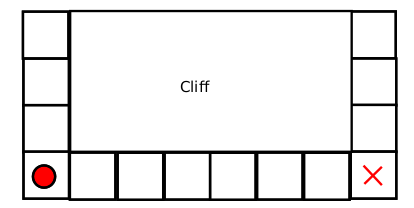
\includegraphics[max size={200}{200}]{report/assets/envs/cliff_real.png}
    \caption{Modified Cliff-Walking Domain}
    \label{fig:cliff-real}
  \end{subfigure}
  \hfill
  \begin{subfigure}{0.45\textwidth}
    \centering
    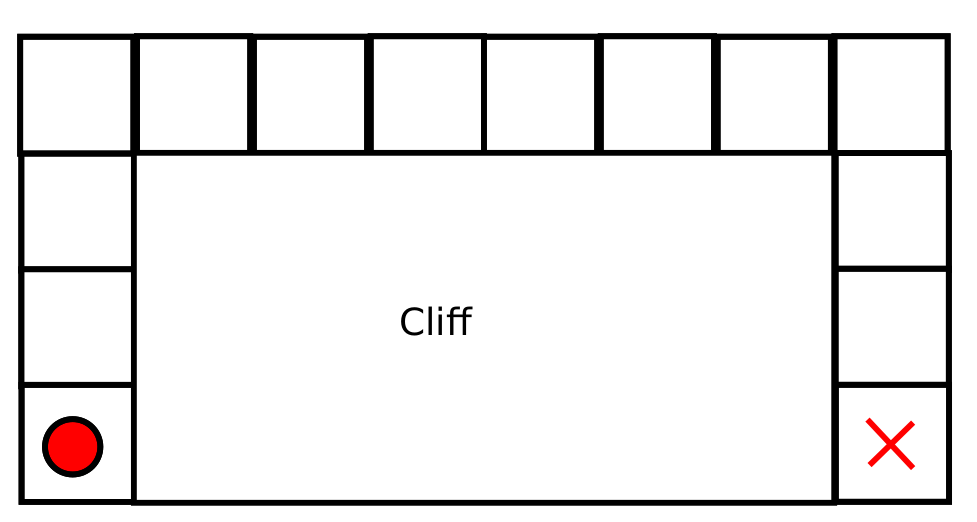
\includegraphics[max size={200}{200}]{report/assets/envs/cliff_model.png}
    \caption{Agent's Model}
    \label{fig:cliff-model}
  \end{subfigure}
  \caption{Comparison of Modified Cliff-Walking Domain and Agent's Model}
  \label{fig:cliff-comparison}
\end{figure}


\\Assuming an implementation of our framework, where reasonable Meta Actions are embedded, that allow the agent to hypothesise changes to transitions and rewards originating in the current state, and targeting an adjacent state. 
Initially, the most beneficial changes to the model would be to remove the cliff across the bottom row, as shown in Figure \ref{fig:cliff-hyp-1}. The agent then attempts to follow the plan going across the bottom of the grid, after which it realises that the hypotheses were correct. The planner may make further hypotheses which lead to the agent trying alternate paths, for instance hypothesising that the cliff is not present across the second row and that the reward through that row is increased; meaning that it would be a better path than the previous one. This process continues, with the planner making hypotheses and the agent verifying them, until no more hypotheses can be made, or the agent runs out of planning steps, after which the model-free learning takes over, and the produce policy matches the initial plan.

\begin{figure}[h!]
    \centering
    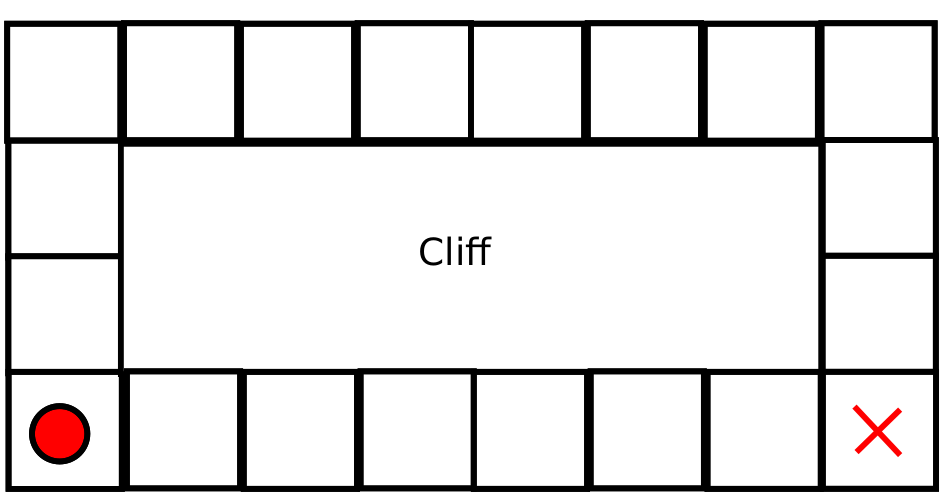
\includegraphics[max size={200}{200}]
    {report/assets/envs/cliff_hypothesis_1.png}
    \caption{Hypothesised Model}
    \label{fig:cliff-hyp-1}
\end{figure}
\section{Implementations}
The high-level ideas of the framework led to various implementations. The main differences among the implementations lie in the choice of planning algorithm, thus how the planning algorithm hypothesises changes, the available Meta Actions and the source of reasonable Meta Actions; learned versus embedded. Furthermore, some implementations had simplifications applied to them to deal with specific domains. We note that these implementations are not definitive, and much improvements could be made, but they are designed with the goal of proving the usefulness of Meta Actions. 
% All implementations were developed in Python. Whilst C or C++ would have been a better choice for computational reasons, various RL benchmarking suites are available for Python.
\subsection{RL-A* Meta}
\label{sec:rlam}
This was the initial implementation of the framework. The chosen planner was a basic A* planner, which limited the implementation to deterministic domains. A* was chosen due to ease of implementation and its use of an evaluation function, $f$, which provided a good means of evaluating Meta Actions. As discussed in Section \ref{sec:astar}, the evaluation function, $f$, is the combination of the heuristic function, $h$, and the cost function. For the cost function, it was intuitive to utilise the reward function. Namely, we define the cost of being in a state, $s$, as the sum of inverted rewards that it took to arrive at that state. Namely:
\begin{equation}
\label{eqn:astarval}
f(s_t) = -\sum_{k=0}^{t-1}\Bigg[R(s_k, a_k, s_{k+1})\Bigg] + h(s_t)
\end{equation}
The choice of heuristic, $h$, relies on domain specific knowledge, therefore we do not define it here. However,  it remains that the heuristic must be admissible. At each state, the next one to be expanded is chosen such that it maximises $f$, taking into account the Meta Actions.
\subsection{RL-A* Meta, with short term memory}
\label{sec:342}
This implementation was an extension of RL-A* Meta, which aimed to scale to stochastic domains. The stochastic nature meant that the evaluation function once again needed to be modified, as such:
\begin{equation}
\label{eqn:astarevalsast}
f(s_t) = -\sum_{k=0}^{t-1}\Bigg[(1-T(s_k, a_k, s_{k+1}))R(s_k, a_k, s_{k+1})\Bigg] + h(s_t)
\end{equation}
Since transitions were not guaranteed, the cost was weighted using the probability of the transition not occurring. This meant that transitions with a higher probability of occurring were preferred.
% \\ The Meta Actions that were available to the planner allowed it to increase/decrease transition probabilities and increase/decrease rewards for state-action-state triples. Reasonable meta actions were embedded in the model by-hand. 
To ensure feasibility of Meta Actions, a table was maintained which kept track of which actions had been called on which state-action-state triples within the previous $N$ episodes; we refer to this as the short-term memory. This encouraged the agent to try Meta Actions again that it had tried in the past, but "forgotten" that it had done so; if it got unlucky previously due to stochasticity, it could try again and discover a good policy it may not have been able to discover before.
\subsection{RL-VI Meta}
The main problem with the RL-A* agents is the reliance on a good heuristic function, which can be difficult to design and hence, they are limited to domains where a good heuristic function can be easily designed.
Therefore, this implementation aims to deal with varying domains. We opted for planning by dynamic programming, namely through Value Iteration (VI). VI was chosen because it allowed for us to easily evaluate plans through the Value Function. We chose VI over Policy Iteration, as it is generally faster, and we needed to perform it many times. Despite its nature, in our setting repeatedly performing VI is not too expensive, as real and hypothetical changes to the model are not too different, which means that it can converge in few iterations. We used a slightly modified version of VI that allowed it to evaluate the Meta Actions. Namely the updated rule was modified as such:
\begin{equation}
\label{eqn:meta_vi}
    V(s) = \max_a \sum_{s'}\max_{M'}T''(s,a,s')[R''(s,a,s') + V(s')]
\end{equation}
Where $M'=(S,A,T'',R'')$ represents each candidate MDP; this includes the original MDP, and those that can be produced by applying each Meta Action.

\subsection{RL-VI Meta, with learned Meta Actions}
The overall implementation is the same as RL-VI Meta, except Meta Actions are learned and obtained through experience, rather than embedded by-hand in the model. Meta Actions are learned when a discrepancy is noticed between the model and the real environment. For instance, when a reward is received that wasn't expected, a Meta Action is learned that increases reward to the value of the unexpected reward. Furthermore, when a transition is experiences that is unexpected, a Meta Action is learned that enables the discrepancy to be emulated; for instance, if the agent expects to move a single state vertically on an "UP" action, but it actually moves to the right, then it will learn to increase the transition probability of moving right on the "UP" action.


% A Meta Action is learned when a discrepancy is noticed between the model and the real environment. When a reward is received for a state-action-state triple that is not expected by the model, a Meta Action is learned to modify the reward function to produce this reward. When a transition occurs that is not expected by the model, a Meta Action is learned that allows the transition function to be modified elsewhere, in the same way. For example, in the Cliff-Walking domain in Figure \ref{fig:cliff-real}, the agent expects taking the "UP" action in a state to move it a single state upwards, if it actually occurs that the agent is moved two states upwards, then the agent will learn a Meta Action that enables the transition probability of moving upwards twice to be increased.


% In the context of rewards, this was as simple as adding a Meta Action for each different reward received. IN the case of transitions, if an action "UP" is taken, which the model expects to move the agent a single state in the upward direction, but actually moves the agent two states upwards, then the agent learns the Meta Action that adds a transition to move two states upwards on the "UP" action. 